\begin{slide}{６．６　立体の体積}
\begin{itemize}
\item　下図の立体の$x=a$から$x=b$までの断面積を$S(x)$とすると、$x$から$x+dx$までの体積は
\begin{figure}[h]
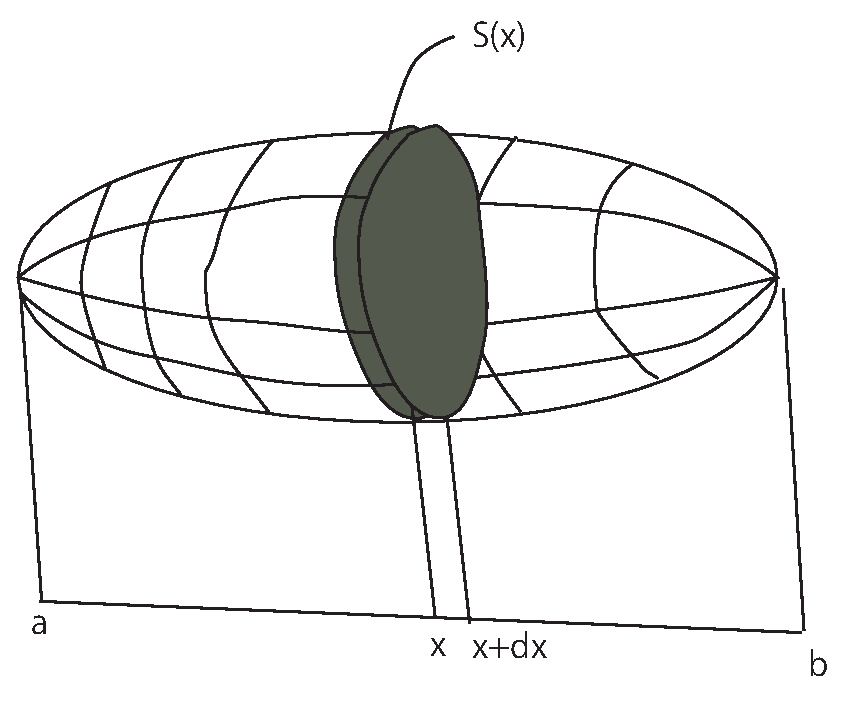
\includegraphics[width=4cm]{calculus12/vol.eps}
\end{figure}
\begin{equation}
\Delta V = S(x)dx \nonumber
\end{equation}
したがって体積$V$は
\begin{equation}
V = \int_a^b S(x)dx \label{eq:vol}
\end{equation}
\end{itemize}
\end{slide}
\begin{slide}{定理６.１２}
$y=g(x) \geqq 0$を$x$軸回りに回転して得られる立体の$a\leqq x \leqq b$の部分の体積$V$は
\begin{equation}
V = \pi \int_a^b g(x)^2 dx \nonumber
\end{equation}
\begin{figure}[h]
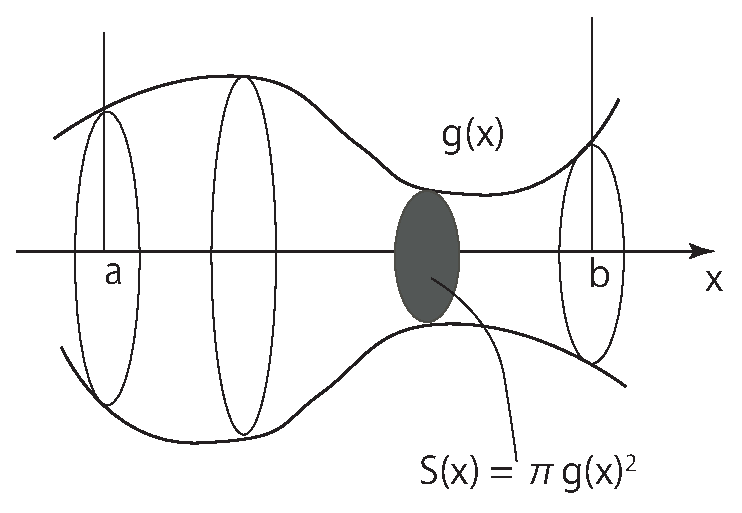
\includegraphics[width=5cm]{calculus12/rot.eps}

$x$の位置での断面積は$S(x)=\pi g(x)^2$なので、式(\ref{eq:vol})を適用。
\end{figure}
\end{slide}
\begin{slide}{例題６．８}
\begin{itemize}
\item $xy$平面の(0, 2)を中心とし半径1の円を$x$軸周りに回転してできる立体（トーラス:torus)の体積を求めよ。
\begin{figure}[h]
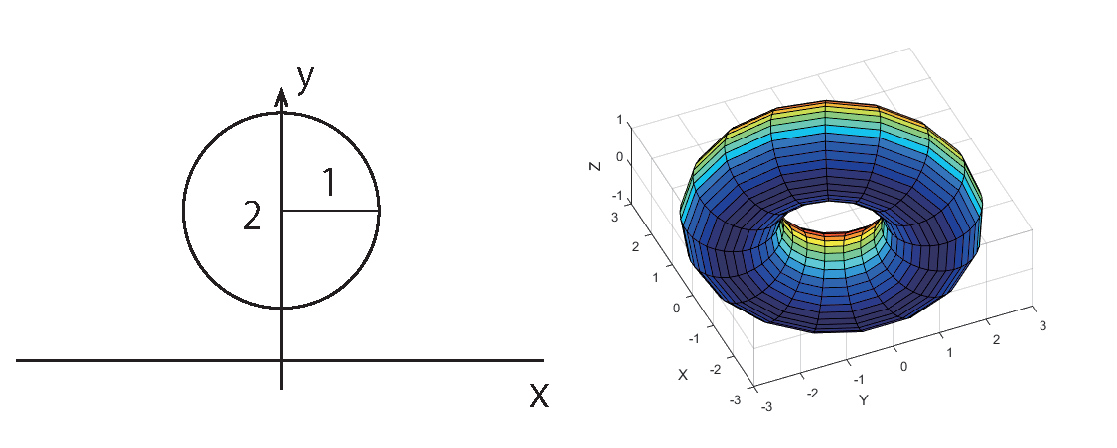
\includegraphics[width=5cm]{calculus12/torus.eps}
\end{figure}
\item 解答例
円の上半分と下半分の方程式はそれぞれ以下となる。
\begin{equation}
y_u(x) =\sqrt{1-x^2} + 2, \qquad y_d(x) = -\sqrt{1-x^2}+2 \nonumber
\end{equation}
\begin{eqnarray}
&& V = \pi \int_{-1}^{1} y_u^2 - y_d^2 dx \nonumber \\
&=& \pi \int_{-1}^1 (\sqrt{1-x^2}+2)^2 - (-\sqrt{1-x^2}+2)^2dx \nonumber \\
&=& 8\pi \int_{-1}^1 \sqrt{1-x^2} dx \label{eq:torus}
\end{eqnarray}
\end{itemize}
\end{slide}
\begin{slide}{例題６．８（２）}
$x=\sin{\theta}$と置換すると、$\frac{dx}{d\theta}=\cos{\theta}$なので
\begin{equation}
\int_{-1}^1 \sqrt{1-x^2} dx = \int_{-\pi/2}^{\pi/2} \cos^2{\theta}d\theta \nonumber
\end{equation}
加法定理から$\cos^2{\theta} = \frac{1+\cos{2\theta}}{2}$なので
\begin{equation}
\int_{-1}^1 \sqrt{1-x^2} dx = \int_{-\pi/2}^{\pi/2} \frac{1}{2} d\theta= \frac{\pi}{2} \label{eq:double}
\end{equation}
式(\ref{eq:double})を式(\ref{eq:torus})に代入して
\begin{equation}
V = 4\pi^2 \nonumber 
\end{equation}
\end{slide}
\begin{slide}{問題６．６}
\begin{itemize}
\item 定積分を用いて底面の半径$r$, 高さ$h$の直円錐(底面の円の中心と頂点とを結ぶ線が底面に垂直である円錐)の体積を求めよ
\item 定積分を用いて半径$r$の球の体積を求めよ
\end{itemize}
\end{slide}
\begin{slide}{６．７　曲線の長さ}
\begin{itemize}
\item $x,y$平面において、曲線$C$の上の点$(x,y)$が変数$t$の関数によって
\begin{equation}
x=f(t), \qquad y=g(t) \nonumber 
\end{equation}
の形に表されるとき、これを$C$のパラメータ表示といい、$t$をパラメタ（媒介変数: parameter)という。
\item 例：原点$O$を中心とし半径$r$の円のパラメタ表示は

\begin{equation}
x = r\cos{\theta}, \qquad y=r\sin{\theta} \quad (0\leqq \theta \leqq 2\pi) \nonumber
\end{equation}
\end{itemize}
\end{slide}
\begin{slide}{曲線の長さ（２）}
\begin{itemize}
\item パラメタ$t$が$t+dt$に動く時の$x,y$は$f(t), g(t)$から$f(t+dt), g(t+dt)$に動くことになる。テイラー展開すると
$f(t+dt) = f(t)+f'(x)dt$, $g(t+dt) = g(t)+ g'(t)dt$であり、曲線の伸び分は$\sqrt{f'(t)^2 + g'(t)^2}dt$となる。
\begin{figure}[h]
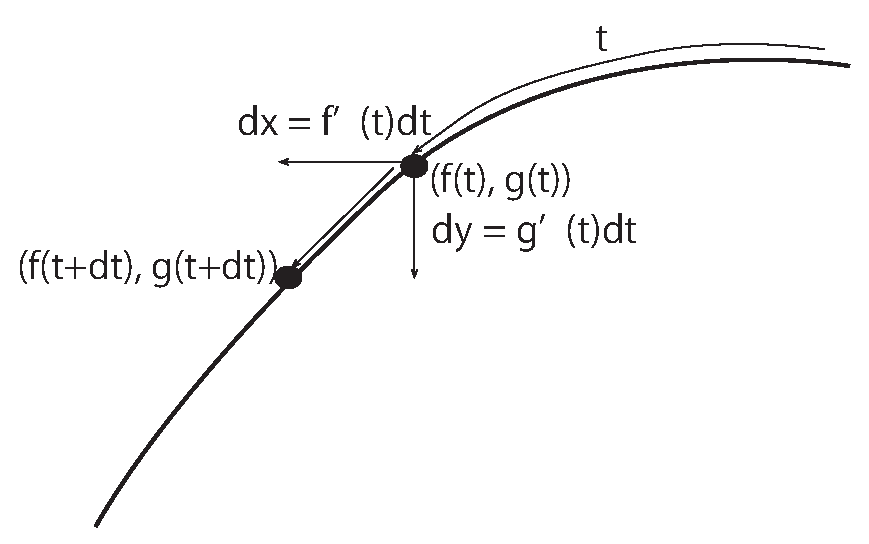
\includegraphics[width=5cm]{calculus12/curv.eps}
\end{figure}
\item $a \leqq t \leqq b$の長さ$l$は
\begin{equation}
l = \int_a^b \sqrt{f'(t)^2 + g'(t)^2} dt \nonumber
\end{equation}
\end{itemize}
\end{slide}
\begin{slide}{曲線の長さ：例}
\begin{itemize}
\item 原点$O$を中心とし半径$r$の円のパラメタ表示は
\begin{equation}
x = r\cos{\theta}, \qquad y=r\sin{\theta} \quad (0\leqq \theta \leqq 2\pi) \nonumber
\end{equation}
であり、$0 \leqq \theta \leqq \pi$の曲線の長さは
\begin{eqnarray}
&& \int_0^{\pi} \sqrt{r^2\sin^2{\theta} + r^2\cos^2{\theta}} d\theta \nonumber \\
&=& \int_0^{\pi} r d\theta = \left[r\right]_0^{\pi} = \pi r \nonumber 
\end{eqnarray}
\end{itemize}
\end{slide}

\begin{slide}{曲線の長さ：補足}
\begin{itemize}
\item　$x,y$平面上の曲線がパラメタを用いずとも$y=g(x)$で求められる場合には $x=t$と考えて
\begin{equation}
f'(t) = 1 \qquad g'(t) = g'(x) = \frac{dy}{dx} \nonumber
\end{equation}
となるため以下となる。
\begin{equation}
l = \int_a^b \sqrt{1+\left(\frac{dy}{dx}\right)^2} dx \nonumber
\end{equation}
\end{itemize}
\end{slide}
\begin{slide}{例題６．１２}
\begin{itemize}
\item $y= \frac{e^x + e^{-x}}{2}$で与えられるとき、$-2 \leqq x \leqq 2$の曲線の長さを求めよ。
\item 解答例: $\frac{dy}{dx} = \frac{e^x - e^{-x}}{2}$なので
\begin{eqnarray}
l &=& \int_{-2}^2 \sqrt{1+\frac{e^{2x} + e^{-2x} - 2}{4}} \nonumber \\
&=& \int_{-2}^2 \sqrt{\frac{e^{2x} + e^{-2x}+2}{4}} = \int_{-2}^2 \frac{e^x + e^{-x}}{2} dx \nonumber \\
&=& \frac{1}{2} \left[e^x - e^{-x}\right]_{-2}^2 = e^2 - e^{-2} \nonumber
\end{eqnarray}
\end{itemize}
\end{slide}
\begin{slide}{例題６．８ トーラス（３）}
媒介変数$\theta$を導入
\begin{figure}[h]
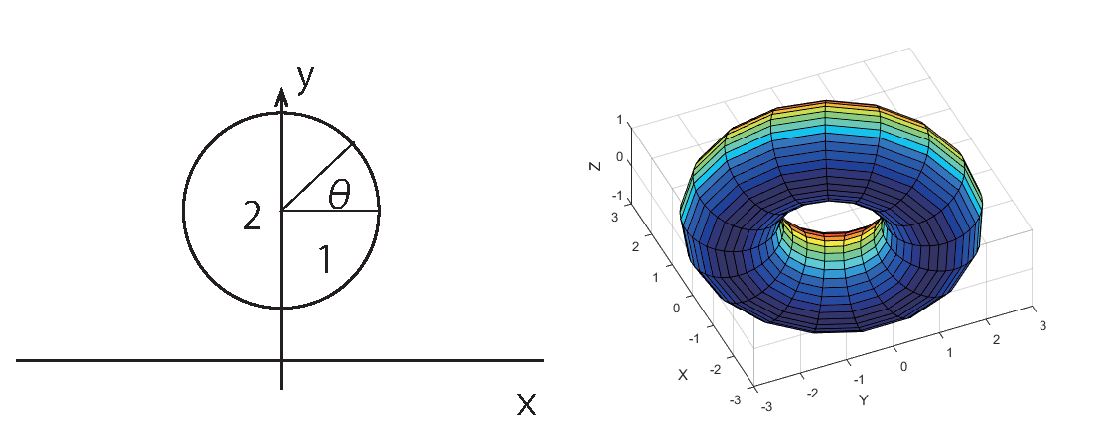
\includegraphics[width=5cm]{calculus12/torus2.eps}
\end{figure}
$\theta$と$x$の関係は
\begin{equation}
x=\cos\theta, \qquad \frac{dx}{d\theta} = -\sin\theta \nonumber 
\end{equation}
$\theta$の時のトーラスの断面積$S$は
\begin{equation}
S =\pi (2+\sin\theta)^2 - \pi(2-\sin\theta)^2 = 8\pi \sin\theta \nonumber
\end{equation}
なので体積$V= \int_{-1}^1 8\pi\sin\theta dx = -8\pi\int_{\pi}^{0} \sin^2\theta d\theta = 8\pi\int_{0}^{\pi} \sin^2\theta d\theta$ 、加法定理を利用して
\begin{equation}
V = 8\pi \int_{0}^{\pi} \frac{1-\cos{2\theta}}{2} dx =4\pi^2 \nonumber
\end{equation}
\end{slide}
\begin{slide}{回転体の体積}
$y=x^2$の関数を$y=x$を中心に$0 \le x \le 1$間で回転させて,できる立体の体積を求めよ。
\begin{figure}[h]
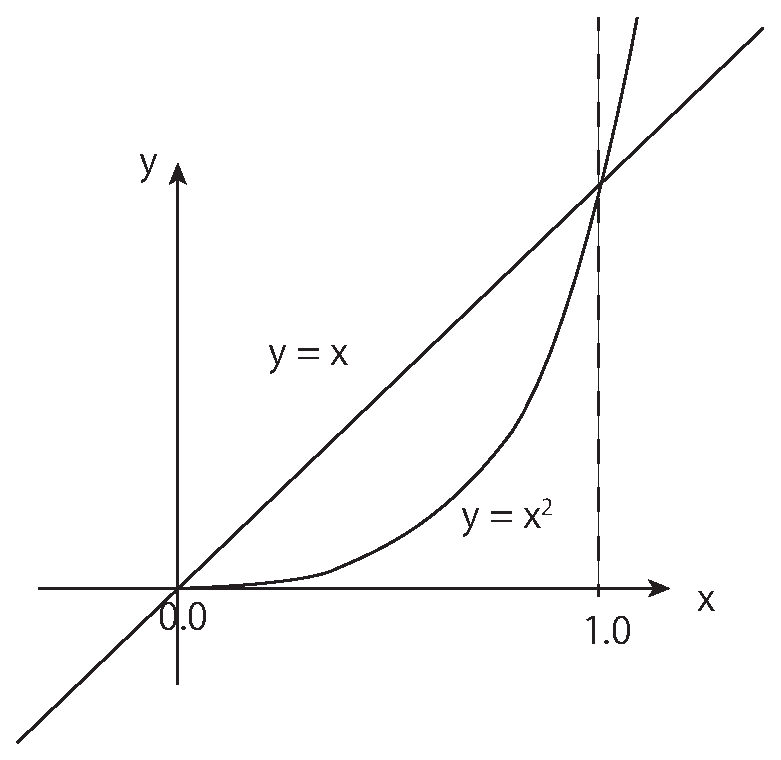
\includegraphics[width=5cm]{calculus12/umb.eps}
\end{figure}
\end{slide}
